\section{Introduction}

\subsection{Background}
In today's increasingly digitized economy, businesses and individuals generate enormous volumes of paper receipts on a daily basis. From retail stores and restaurants to hospitals and government agencies, receipts serve as critical records of financial transactions. Yet despite the digital revolution transforming nearly every other aspect of commerce, the processing of these physical documents remains surprisingly manual in many organizations. Accountants still key in figures by hand, expense management teams sort through stacks of paper, and auditors cross-reference printed records against digital ledgers, which is a workflow that is both tedious and prone to human error.
Automating this process begins with a fundamental Computer Vision task: detecting and localizing text within document images. Before any meaningful information can be extracted from a receipt, a system must first be able to identify where text appears on the page by drawing bounding boxes around each word or phrase and correctly reading its content. This is far from straightforward in practice. Scanned receipts often suffer from skewed alignment, inconsistent font sizes, varying print quality, and cluttered layouts where prices, item descriptions, addresses, and merchant details are packed into a compact space with no standardized structure across vendors.

Optical Character Recognition (OCR) combined with text detection has emerged as the foundational approach for tackling this challenge. Modern deep learning models are now capable of not only pinpointing the spatial location of text regions through bounding box prediction, but also transcribing the text content within those regions to produce structured, machine-readable output from raw document images. The ICDAR 2019 Robust Reading Challenge on Scanned Receipts OCR and Information Extraction (SROIE) was established as a standardized benchmark to drive progress in exactly this area, and its dataset has since become a widely adopted reference for evaluating document text detection systems.
\subsection{Problem Statement}
The core challenge addressed in this project is text detection and recognition on scanned receipt images. We need to identify every text region present in a receipt, draw a precise bounding box around it, and predict the text label it contains. While this may seem like a well-defined task, receipts introduce a number of practical difficulties. Text lines vary in length, orientation, and density. Printed characters can blur, smear, or overlap due to low-quality scanning. Different receipts follow entirely different spatial layouts depending on the issuing merchant, meaning no fixed template can be assumed.

These challenges make it insufficient to apply generic OCR tools without adaptation. A robust text detection system must generalize across diverse receipt styles, handle visual noise gracefully, and produce accurate bounding box predictions that tightly enclose each text instance without missing or merging adjacent regions. Errors at this detection stage directly undermine any downstream processing, making it the most critical step in any automated receipt understanding pipeline.
\subsection{Objectives}
The primary objectives of this project are as follows:

- To develop and implement a pipeline for receipt OCR and information extraction using the ICDAR 2019 SROIE dataset.

- To perform text recognition on the detected regions, producing a predicted label for each bounding box that corresponds to the transcribed text content.

- To evaluate the performance of the implemented approach using the metrics defined by the SROIE challenge, including precision, recall, and F1-score for both the OCR and information extraction tasks.

- To analyze the challenges encountered in processing real-world receipt images and discuss the limitations and potential improvements of the proposed system.
\subsection{Dataset Description}
This project uses the ICDAR 2019 Scanned Receipts OCR and Information Extraction (SROIE) dataset, made publicly available through the official competition repository and mirrored on GitHub by zzzDavid. The dataset consists of 1,000 whole scanned receipt images, each annotated with bounding box coordinates and ground truth text labels for every text region present in the image. The receipts span a wide variety of merchants, layouts, and printing conditions, providing a diverse and realistic benchmark for evaluating text detection and recognition systems on document images. An example scanned receipt is shown below:
\begin{figure}[h]
  \centering
  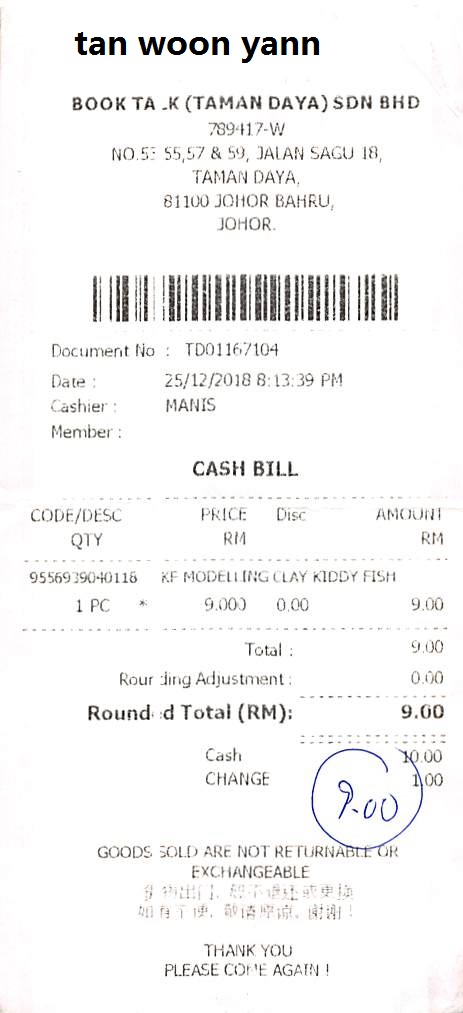
\includegraphics[width=0.4\textwidth]{images/X00016469612.jpg}
  \caption{An example scanned receipt from the SROIE dataset.}
  \label{fig:example_receipt}
\end{figure}
\newpage